\documentclass[10pt,twocolumn,letterpaper]{article}
\usepackage[utf8]{inputenc}  
\usepackage{cvpr}
\usepackage{times}
\usepackage{epsfig}
\usepackage{graphicx}
\usepackage{amsmath}
\usepackage{amssymb}

% Include other packages here, before hyperref.

% If you comment hyperref and then uncomment it, you should delete
% egpaper.aux before re-running latex.  (Or just hit 'q' on the first latex
% run, let it finish, and you should be clear).
\usepackage[breaklinks=true,bookmarks=false]{hyperref}

\cvprfinalcopy % *** Uncomment this line for the final submission

%\def\cvprPaperID{****} % *** Enter the CVPR Paper ID here
\def\httilde{\mbox{\tt\raisebox{-.5ex}{\symbol{126}}}}

% Pages are numbered in submission mode, and unnumbered in camera-ready
%\ifcvprfinal\pagestyle{empty}\fi
\setcounter{page}{1}
\begin{document}

%%%%%%%%% TITLE
\title{Sin City, Classification of Regional Songs in Turkey}

\author{Muhammet Emin Özgür\\
%Institution1 address\\
{\tt\small b21427229@cs.hacettepe.edu.tr}
% For a paper whose authors are all at the same institution,
% omit the following lines up until the closing ``}''.
% Additional authors and addresses can be added with ``\and'',
% just like the second author.
% To save space, use either the email address or home page, not both
\and
Ufuk Umut Şentürk\\
%First line of institution2 address\\
{\tt\small b21427435@cs.hacettepe.edu.tr} \\
\and
Muazzez Şule Karaşlar\\
%First line of institution2 address\\
{\tt\small b21427066@cs.hacettepe.edu.tr}\\
{Machine Learning Lab, Department of Computer Engineering}\\
{Hacettepe University, Ankara, TURKEY}\\
}

\maketitle
%\thispagestyle{empty}
%%%%%%%%% ABSTRACT
\begin{abstract}
  In most cultures we can define a generic type of songs that defines the culture. We can even pinpoint the differences between similar cultures but relatively in a different region which might be city, county or state. This is the point where idea came to classify folk songs in Turkey region by region. Turkey has 7 geographic regions which can be seen as cultural regions. Thus, those regions do not have completely different cultures,but differences are visible which one of them is the regional songs. For instance, tulum, kemençe(endemic musical instruments for Karadeniz) can be heard in Karadeniz songs which are distinguishable from other regions songs. However, some regions have same musical infrastructure which are rhythm, instruments, chords or notes patterns and vocal type which is hard to distinguish for a human being. This one is probably the hardest challenge we will face. Hence, feature extraction is the crucial point for this matter and there are certain features can be used for our classification problem and there are some must be tried before used. We will try to implement and analyze different models and different features for this classification problem.
\end{abstract}
%%%%%%%%% BODY TEXT
\section{Introduction}
\paragraph{}In machine learning most important step is the feature extraction. Just by improving features will increase dramatically for contemporary machine learning models. In the audio feature extraction, current state-of-art is being provided by MIR(Music Information Retrieval) research field. MIR is a huge field that has been under the spotlight since Tzanetakis and Cook released a paper on Music Genre Classification in 2002\cite{genre_classification_tp}. MIR includes audio feature extraction, signal processing, audio analyse etc. Audio feature extraction is what we are interested in MIR research field. We are planning mainly to use features: Chroma-gram, MFCC(Mel-frequency cepstral coefficients), Spectral centroid, Spectral roll-of, Zero-crossing rate, etc. We will also use other features for reference points but these will be the main features.
Machine learning model selection for the job is not without importance. State-of-art models are plentiful, however they are mostly specific for a given problem. In order to find the best classification, we will use various models which will be CNN(Convolutional Neural Network), SVM(Support Vector Machine), K-NN(K Nearest Neighbor). These machine learning models will be implemented with various contemporary features discussed in MIR. Subsequently these will be analysed.   
Analyzing will be last step in our paper. We will gather results after the testing which in a matrix as rows for machine learning models and columns for features. Best model and features will be apparent after the testing is done. Confusion matrix will be constructed by using our best model and features.   

%-------------------------------------------------------------------------
\section{Related Works}

\paragraph{}In this paper, classification problem is more specific than any other work. since Tzanetakis and Cook presented music genre classification\cite{genre_classification_tp}, a lot of work has been done. 
For Audio processing and analyzing, it is hard to build-up a reliable feature extractor system for audio seems to be a more challenging task than classification problem.
For this purpose some researches have been done about features extraction such as; MFCC\cite{mffc}, Chromogram\cite{chroma}, Zero-crossing rate, Spectral-Centroid\cite{spectral_centroid}.
\paragraph{}The most known study for folk song classification which is based on region has been done for China. On paper in interest, 74 features have been extracted from audio files of the songs, and classified by an audio classifier on SVM which is one of our concern. Research shows usthat SVM without feature selection is a very effective classification method with the combination of 13-dimension MFCC and 10-dimension without feature selection. It points us to post processing and segmentation plays key role in here. Other research is called "Regional Classification of Traditional Japanese Folk Songs" by Akihiro KAWASE, Akifumi TOKOSUMI has been made. That research use music corpora consisting of 202,246 tones from 1,794 song pieces from 45 prefectures in Japan which is big enough.

\paragraph{}In another research\cite{feature_extraction_automatic_cnn}, presented a methodology to automatically extract musical patterns features from audio music using the CNN which is easy to use for feature extractors, it because need minimal prior knowledge to construct. Some other paper uses\cite{genre_classification} various machine learning algorithms that are including k-nearest neighbor (kNN), k-means, multi-class SVM, and neural networks to classify the following four genres: classical, jazz, metal, and pop and only Mel Frequency Cepstral Coefficients (MFCC) is used to characterize data.
Using CNN is become quite popular in other ML fields with each other. Qiuqiang Kong, et al\cite{genre_cnn} stated that many manual-selected features such as MFCC have been applied to music processing but they are not effective for music genre classification. In their work, it is presented an algorithm based on spectrogram and CNN and compared with MFCC, the spectrogram contains more details of music components such as pitch, flux, etc. 


%-------------------------------------------------------------------------
\section{Methodology}

\subsection{Data Set}
\paragraph{}We have gathered our data from youtube playlist. There are various regional playlist which we have found with quick search\cite{data_set}. We obtained these in ogg format and as smallest bitrate as possible we can find in order to save space. JDownloader\cite{jdownloader} used to download these playlist with ease. Each download placed in respective folder for label in their classification. In these playlist there might be noise such as given song might not be in that regional as suggested in the name of the playlist. These will be most likely a miniscule noise. Moreover we will add more songs in the data set, hence the noise will be smaller with each growth of the data set. 

\subsection{Features}
\paragraph{}As hitherto cited, MFFC, Spectral Centroid, Spectral roll-of, Zero-crossing rate\cite{genre_classification_tp} are main focus in this paper. Librosa\cite{librosa} is used for feature extraction library. It is not the fastest library, it is only used because of convenience. These features will have tremendous dimension space which would need dimension reduction with PCA(Principle Component Analysis) and feature selection techniques. 
\begin{figure}[t]
  \begin{center}
  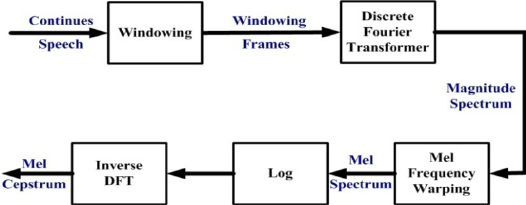
\includegraphics[width=0.8\linewidth]{images/mfcc_calc.png}
  \end{center}  
     \caption{MFCC Calculation Process.\cite{mfcc_calc}}
  \label{fig:mffc}
  \label{fig:onecol}
\end{figure}
\paragraph{} Above figure shows us the calculation steps of MFCC\cite{mfcc_calc}. MFCC is a convenient feature used in speak recognition, signal processing. Alternatively, spectral centroid feature is proposed and used widely. Below figure shows spectral centroid.\cite{spec_centroid}
\begin{figure}[t]
  \begin{center}
  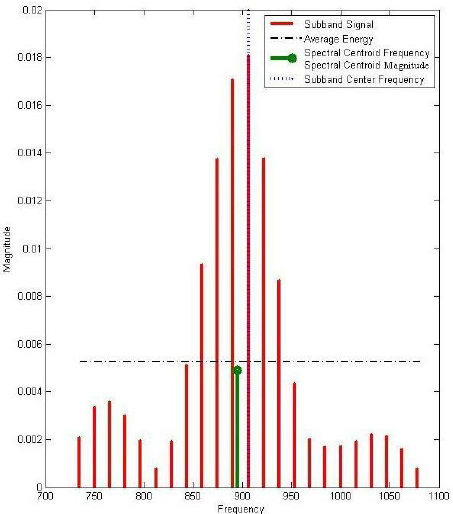
\includegraphics[width=0.8\linewidth]{images/spec_centroid.png}
  \end{center}  
     \caption{Subband signal, average energy, spectral centroid frequency and spectral centroid\cite{spec_centroid}.}
  \label{fig:mffc}
  \label{fig:onecol}
\end{figure} 

\subsection{Classification}
\paragraph{}We will implement 3 classification model, namely SVM, CNN, K-NN. In the CNN implementation we will use tensorflow. CNN architecure will have 2 convolution layer in which each layer followed by max pooling and drop out. However it is still in progress, hence it is subject to change. SVM and K-NN will be implemented by scikit-learn python module.

\section{Feature Works}
\paragraph{}Implementation of our classification will be our next step. Following our implementation we will test it with our focused features and along-the-way features that we thought might improve accuracy. Feature extraction libraries might change, following that if the new library does not have our features, they might change too\textemdash little chance. However we will not change library if we might loose critical feature we have found out after our tests. 


{\small
\bibliographystyle{ieee}
\bibliography{egbib}
}

\end{document}
